\documentclass[tikz, border=3mm]{standalone}
\usepackage{tikz}
\usetikzlibrary{arrows.meta, positioning} % For arrow tips and relative positioning

\begin{document}
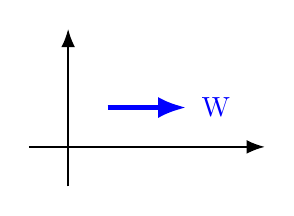
\begin{tikzpicture}[
    >=Latex % Set default arrow tip style
]

    % Axes
    \draw[->, thick] (-0.5, 0) -- (2.5, 0); % x-axis
    \draw[->, thick] (0, -0.5) -- (0, 1.5); % y-axis

    % Define vector points
    \coordinate (Wstart) at (0.5, 0.5);
    \coordinate (Wend)   at (1.5, 0.5);

    % Draw Vector W (make it quite thick)
    \draw[->, blue, ultra thick] (Wstart) -- (Wend);

    % Label W
    \node[blue, right=2pt of Wend] {W}; % Position label right of the endpoint

\end{tikzpicture}
\end{document}